\subsection{Purpose}

During the COVID-19 pandemic in order to reduce the of transmission of the virus governments have introduced various measures aimed to reduce to a minimum close contacts between people, these measures include social distancing and lockdowns.

During lockdowns people can leave their habitations only for essential needs such as grocery shopping, which makes supermarkets a gathering spot where the virus could spread and potential danger for the people visiting.

For this reason the access to essential activities should be limited to lower the density of people inside the activities and allow keeping distances effectively and mitigate the risk.

However this is not of trivial execution, because in order to serve the same amount of people, with reduced maximum capacity, the clients need to access the activity distributed over a longer timespan than regular operation. This means that if too many people want to access the store in a given moment, some people will be left out and this will result in a line of people waiting to enter the store.

This is a hazard in and of itself since people outside will stay for a prolonged amount of time in close proximity with each other while waiting for their turn.

The problem of forming lines can be mitigated by handing a number to each client and having people enter in order of arrival, this approach, while better than queueing, still requires all clients to go to the store and take a ticket, and while they won't need to stay in a queue, people will still need to wait close to the activity.

This application aims to provide a digital alternative to the "handing numbers" approach and improve it by allowing people to take their number online, this way people only need to go to the store when it's their turn to enter and they won't need to hang around the building.

The product will also allow store managers to effectively monitor the entrances by scanning a QR code associated with the "number" to ensure the safety limits are being followed.

Additionally to the lining up mechanism the application will allow customers to book a visit in the future, which will improve the distribution of customers during the day and the week, since they will be able to choose a less crowded time slot.

CLup will also allow users to choose the approximate time of their visit and the category of items they wish to buy, which allows making more accurate predictions of the waiting times and, by knowing the areas that they will visit, to better utilize the space in the building, while respecting health and safety measures.

\subsubsection{Goals}

\begin{description}
    \item [G1]  Users shall be able to enqueue in the waiting list for the Shop
    \item [G2]  Users shall be able to book a visit to the Shop
    \item [G3]  Users shall be provided with an estimate of the waiting time for a Shop
    \item [G4]  Users should be reminded about considering the time needed to travel to the Shop
    \item [G5]  Users shall be able to specify the categories of items they intend to buy 
    
    \item [G6]  Third parties shall be able to add Users to the waiting list for the Shop on their behalf
    \item [G7]  Third parties shall be able to book a visit to the Shop on the Users' behalf
    \item [G8]  Third parties shall be able to verify the presence of a User in the current waiting list, or in the bookings for the current time slot
    \item [G9]  Third parties shall be able to monitor the number of visits to the Shops, to ensure compliance with the laws
    \item [G10] Third parties shall be able to retrieve data about booked visits, including the categories of items requested by each User 
    
\end{description}
\subsection{Scope}

Using the "The World and The Machine" model by M. Jackson we can give an overall description of the events involved in the project realization, both those which cannot be observed by the system "The World" and those strictly related to the system "The Machine", but also those in common between the two.

\begin{figure}[h]
    \centering
    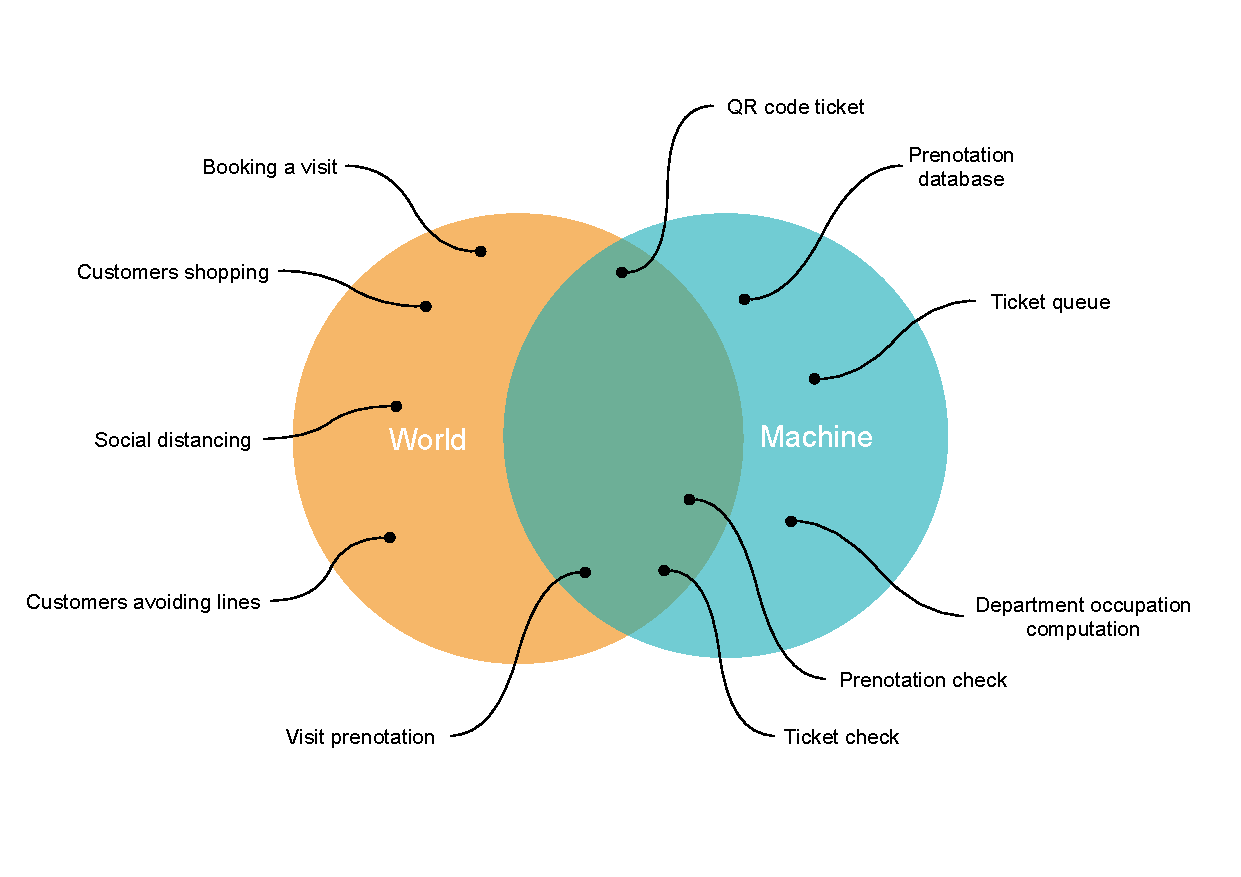
\includegraphics[width=.85\textwidth]{Images/world-machine.pdf}
    \caption{\label{fig:world_machine} World Machine diagram}
\end{figure}


\subsection{Definitions, Acronyms, Abbreviations}
\subsubsection{Definitions}
\begin{description}
    \item [Third party company] A company that wants to use our services.
    {\todo
        \item \huge TODO
    }
\end{description}
\subsubsection{Acronyms}
\begin{description}
    \item [RASD] Requirement Analysis and Specification Document. 
    \item [API] Application Programming Interface.
    {\todo
        \item \huge TODO
    }
\end{description}
\subsubsection{Abbreviations}
\begin{description}
    \item [Third party] A company that wants to use our services.
    \item [{[Gn]}] n-goal. 
    \item [{[Dn]}] n-domain assumption. 
    \item [{[Rn]}] n-functional requirement. 
\end{description}

\subsection{Revision history}
{
\todo
\begin{description}
    \item[v. 1.0 - 44/55/666] Initial release
	\item[v. 1.1 - 44/55/666] Fixed return values in sequence diagrams; removed unnecessary Location class from class diagrams; removed unnecessary intermediate state for SpecificRequest and GroupRequest state diagrams
	\item[v. 1.2 - 44/55/666] Adjusted User's fields in class diagrams; adjusted target Android API; removed a duplicate line in requirements
\end{description}
}
\subsection{Reference documents}
{\todo
\begin{minipage}{\textwidth}
    \begin{description}
        \item [BEEP channel] - Mandatory Project Assignment
        \item [The world \& the machine] - M. Jackson, P. Zave
    \end{description}
    \end{minipage}
}
\subsection{Document structure}
This document is structured in four main chapters, that are as follows:
\begin{enumerate}
	\item The first chapter serves as an introduction and an overview to the project, describing the main reasons for its development, its goals together with a brief informal description of it.

	\item The second chapter serves as a more formal description of the project: it includes class diagrams, state machine diagrams, and it gives details on the shared phenomena and domain models. Class diagrams give a big picture description on how the system should be structured, while state machine diagrams focus on the more relevant entities of the model. Here are also presented all the requirements and domain assumptions the system in project must fulfill and take into considerations, in order to achieve the goals; they are presented each one after the goal it is relevant to.

	\item The third chapter presents the specific requirements: use cases and the design constraints the system must satisfy. The use cases are described using natural language, while the constraints are pictured with sequence/activity diagrams. A mockup is also shown as a general idea of how the end product should be, in terms of design and functionalities offered to the end user.

	\item The fourth and last chapter is a formal analysis of the model, made through the use of the open source Alloy language and analyzer, including a graphic representation of it obtained from Alloy Tool.
\end{enumerate}
